\documentclass[a4paper]{article}

\usepackage[margin=3cm]{geometry}

% the last of the arguments is the default language
\usepackage[ngerman,english]{babel}

% header and footer
\usepackage{fancyhdr}

\usepackage[utf8]{inputenc}

\usepackage[pdftex]{graphicx}

% we need to use 'minipage' for figures (instead of the 'figure' environment).
% hence, we need the 'captionof' command (part of the 'caption' package).
\usepackage{caption}

\usepackage{xcolor}

% code background
\definecolor{code}{gray}{.95}

% create diagrams
\usepackage{tikz}

%\usepackage{hyperref}
\usepackage[pdftex,
            pdfauthor={Secure by Default, Inc.},
            pdftitle={Penetration Test Report},
            pdfsubject={Example Pentest},
            pdfkeywords={},
            pdfproducer={LaTeX},
            pdfcreator={pdflatex}]{hyperref}
            
% inline code
\newcommand{\passthrough}[1]{\colorbox{code}{\lstset{mathescape=false}#1}}

% define level-4 section
\usepackage{titlesec}
\setcounter{secnumdepth}{4}
\titleformat{\paragraph}
  {\normalfont\normalsize\bfseries}{\theparagraph}{1em}{}
  \titlespacing*{\paragraph}
  {0pt}{3.25ex plus 1ex minus .2ex}{1.5ex plus .2ex}

% Pandoc uses '\tightlist' inside list environments
\def\tightlist{}

% disable indentation of first line of paragraphs
\usepackage{parskip}

% nice code listings
\usepackage{listings}
\lstset{
  backgroundcolor=\color{code},
  basicstyle=\footnotesize\ttfamily,
  upquote=true,
  linewidth=\textwidth,
  breaklines,
  breakatwhitespace,
  frame=single,
  numbers=none,
}

% severity gauge
%
%              7
% ||||||||||||||......
% 0                 10
\newcommand{\severitygauge}[3][1]{
  \begin{tikzpicture}[scale=#1]
    % bounding box
    \path (-3,0) (13,0);

    % empty rectangle
    \filldraw[fill=white, draw=black] (0, -0.1) rectangle (10, 0.1);

    % filled rectangle, showing the gauge's measurement
    \filldraw[fill=black, draw=black] (0, -0.1) rectangle (#2, 0.1);

    % range of the gauge
    \path (0, -0.2) node[anchor=north]{0};
    \path (10, -0.2) node[anchor=north]{10};

    % the gauge's measurement as text
    \path (#2, 0.2) node[anchor=south]{#3};
  \end{tikzpicture}
}

% minimal severity gauge: without range and textual measurement.
% horizontal
\newcommand{\minmalseveritygaugeH}[2][1]{
  \begin{tikzpicture}[scale=#1, baseline=-0.5ex]
    \filldraw[fill=white, draw=black] (0, -0.3) rectangle (10, 0.3);
    \filldraw[fill=black, draw=black] (0, -0.3) rectangle (#2, 0.3);
  \end{tikzpicture}
}

% minimal severity gauge: without range and textual measurement.
% vertical
\newcommand{\minmalseveritygaugeV}[2][1]{
  \begin{tikzpicture}[scale=#1]
    \path (0, 0) (0, 12); % bounding box
    \filldraw[fill=white, draw=black] (-0.5, 0) rectangle (0.5, 10);
    \filldraw[fill=black, draw=black] (-0.5, 0) rectangle (0.5, #2);
  \end{tikzpicture}
}

% conditionals (in macros)
\usepackage{etoolbox}

\newcommand{\highlight}[3]{
  \ifstrequal{#2}{#3}{\framebox{#1}}{#1}
}

\newcommand{\CVSStwo}[7]{
  \begin{tabular}{ll}
    \textbf{Access Vector} & \textbf{Confidentiality Impact}
    \\
    \highlight{Local}{L}{#2} \hspace{0.5em} \highlight{Adjacent Network}{A}{#2} \hspace{0.5em} \highlight{Network}{N}{#2}
    \hspace{2em}
    &
    \highlight{None}{N}{#5} \hspace{0.5em} \highlight{Partial}{P}{#5} \hspace{0.5em} \highlight{Complete}{C}{#5}
    \vspace{1.5ex}
    \\
    \textbf{Access Complexity} & \textbf{Integrity Impact}
    \\
    \highlight{High}{H}{#3} \hspace{0.5em} \highlight{Medium}{M}{#3} \hspace{0.5em} \highlight{Low}{L}{#3}
    \hspace{2em}
    &
    \highlight{None}{N}{#6} \hspace{0.5em} \highlight{Partial}{P}{#6} \hspace{0.5em} \highlight{Complete}{C}{#6}
    \vspace{1.5ex}
    \\
    \textbf{Authentication} & \textbf{Availability Impact}
    \\
    \highlight{Multiple}{M}{#4} \hspace{0.5em} \highlight{Single}{S}{#4} \hspace{0.5em} \highlight{None}{N}{#4}
    \hspace{2em}
    &
    \highlight{None}{N}{#7} \hspace{0.5em} \highlight{Partial}{P}{#7} \hspace{0.5em} \highlight{Complete}{C}{#7}
  \end{tabular}
}

\newcommand{\CVSSthree}[9]{
  \begin{tabular}{ll}
    \textbf{Attack Vector} & \textbf{Scope}
    \\
    \highlight{Network}{N}{#2} \hspace{0.5em} \highlight{Adjacent}{A}{#2} \hspace{0.5em} \highlight{Local}{L}{#2} \hspace{0.5em} \highlight{Physical}{P}{#2}
    \hspace{2em}
    &
    \highlight{Unchanged}{U}{#6} \hspace{0.5em} \highlight{Changed}{C}{#6}
    \vspace{1.5ex}
    \\
    \textbf{Attack Complexity} & \textbf{Confidentiality}
    \\
    \highlight{Low}{L}{#3} \hspace{0.5em} \highlight{High}{H}{#3}
    \hspace{2em}
    &
    \highlight{None}{N}{#7} \hspace{0.5em} \highlight{Low}{L}{#7} \hspace{0.5em} \highlight{High}{H}{#7}
    \vspace{1.5ex}
    \\
    \textbf{Privileges Required} & \textbf{Integrity}
    \\
    \highlight{None}{N}{#4} \hspace{0.5em} \highlight{Low}{L}{#4} \hspace{0.5em} \highlight{High}{H}{#4}
    \hspace{2em}
    &
    \highlight{None}{N}{#8} \hspace{0.5em} \highlight{Low}{L}{#8} \hspace{0.5em} \highlight{High}{H}{#8}
    \vspace{1.5ex}
    \\    
    \textbf{User Interaction} & \textbf{Availability}
    \\
    \highlight{None}{N}{#5} \hspace{0.5em} \highlight{Required}{R}{#5}
    \hspace{2em}
    &
    \highlight{None}{N}{#9} \hspace{0.5em} \highlight{Low}{L}{#9} \hspace{0.5em} \highlight{High}{H}{#9}
  \end{tabular}
}

\newcommand{\DREAD}[5]{
  \begin{tabular}{lccc}
    \textbf{Damage}          & \highlight{Low}{L}{#1} & \highlight{Medium}{M}{#1} & \highlight{High}{H}{#1} \\
    \textbf{Reliability}     & \highlight{Low}{L}{#2} & \highlight{Medium}{M}{#2} & \highlight{High}{H}{#2} \\
    \textbf{Exploitability}  & \highlight{Low}{L}{#3} & \highlight{Medium}{M}{#3} & \highlight{High}{H}{#3} \\
    \textbf{Affected Users}  & \highlight{Low}{L}{#4} & \highlight{Medium}{M}{#4} & \highlight{High}{H}{#4} \\
    \textbf{Discoverability} & \highlight{Low}{L}{#5} & \highlight{Medium}{M}{#5} & \highlight{High}{H}{#5} 
  \end{tabular}
}

% align columns at decimal points
\usepackage{dcolumn}
\newcolumntype{d}[1]{D{.}{.}{#1}}

% nicer tables
\setlength{\tabcolsep}{10pt} % increase horizontal spacing; default value: 6pt
\renewcommand{\arraystretch}{1.5} % increase vertical spacing; default value: 1
\begin{document}

% header and footer
\pagestyle{fancy}
\fancyhf{} % clear existing header/footer entries

\begin{titlepage}

  \vspace*{\fill}

  \begin{center}
    \makebox[\textwidth]{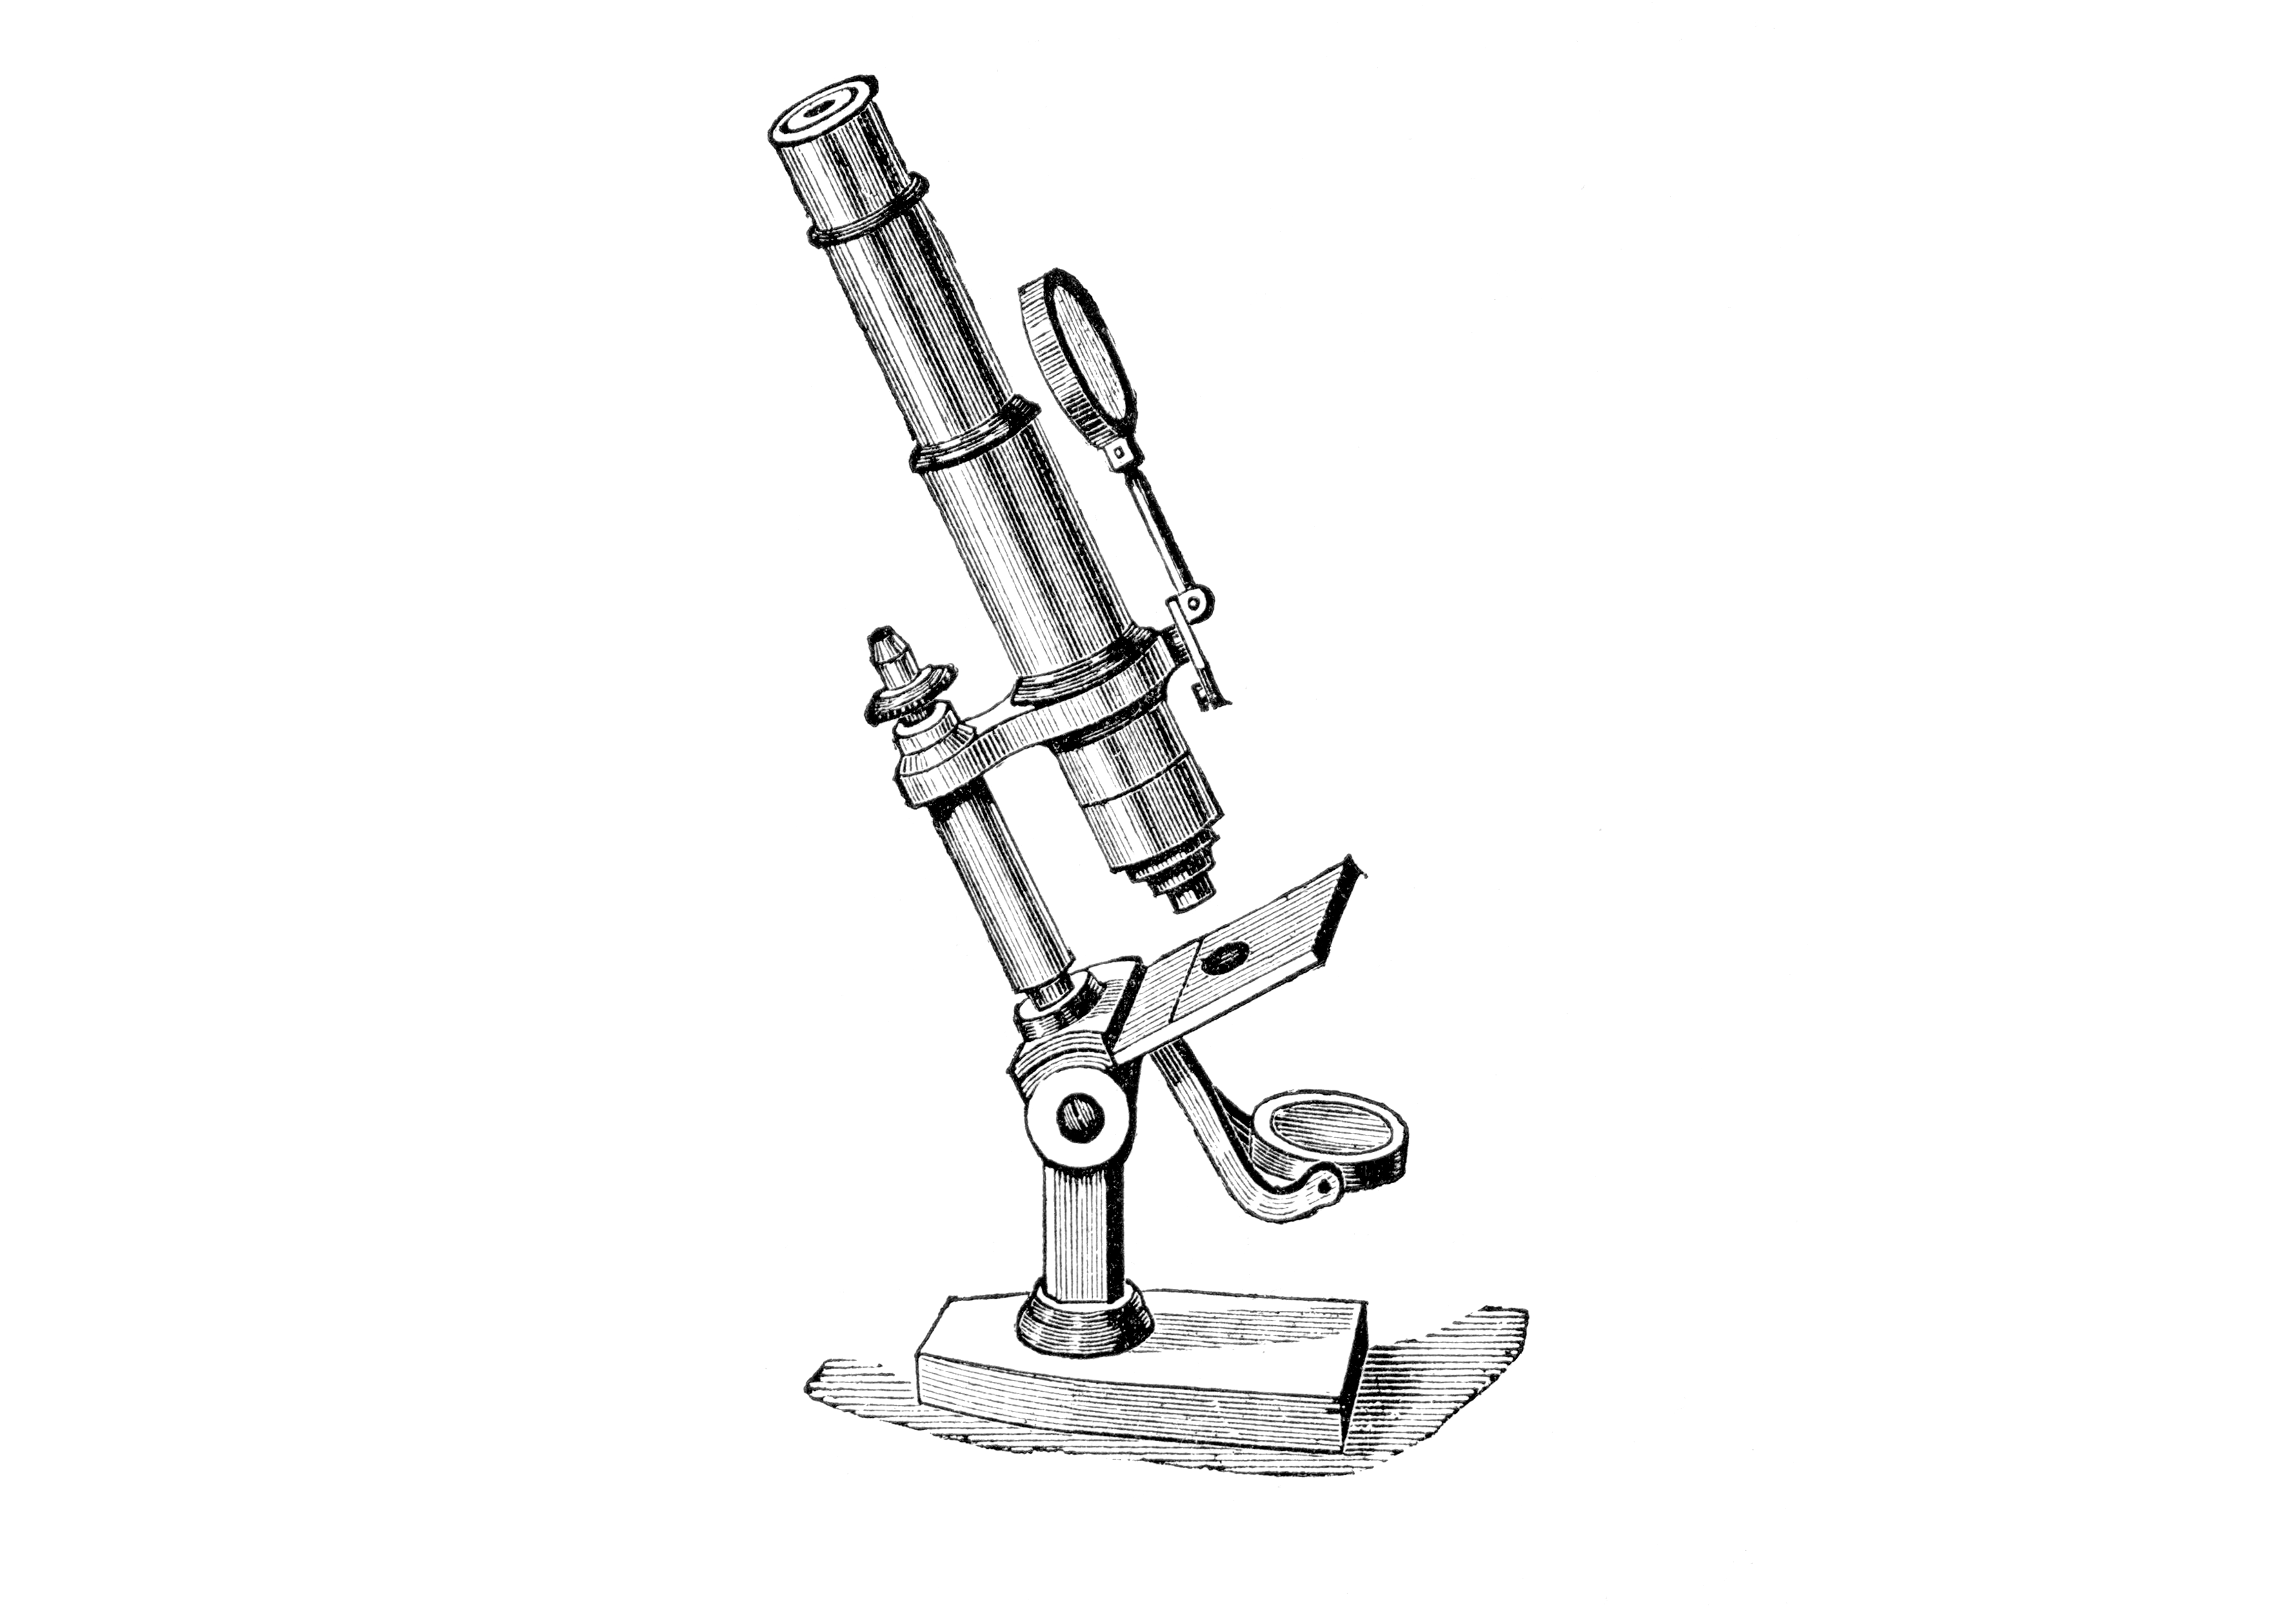
\includegraphics[width=\paperwidth]{templates/title}}
  \end{center}

  \vfill
  
  {
    \Huge \textbf{\MakeUppercase{Penetration Test Report}}
    \vspace{1ex}
  }

  {
    \Large \textbf{Example, Inc.}
    %\vspace{1ex}
  }

  {
    \Large \textbf{Example Pentest}
    %\vspace{1ex}
  }

  yyyy-mm-dd (1.0)
\end{titlepage}

\fancyhead[L]{Example Pentest}
\fancyhead[R]{Confidential}

\fancyfoot[C]{\thepage}

{
  \vspace*{\fill}

  This report is for the sole information and use of Example, Inc.

  \textbf{Secure By Default, Inc.} \\
  \href{tel:+0123456789}{+0 123 456 789} \\
  \href{mailto:contact@sbd.local}{contact@sbd.local} \\
  \href{https://sbd.local/}{https://sbd.local/}
}

\clearpage
\section*{Executive Summary}
%\addcontentsline{toc}{section}{Executive Summary}

Example, Inc.\ (i.e.\ the customer) engaged Secure By Default, Inc.\ to conduct a penetration test on their systems.
In accordance with the customer the following types of penetration tests have been conducted:

\begin{itemize}
      \item pentest against web applications

      \item pentest against IP hosts

  \end{itemize}

Vulnerabilities with severity scores between 6 and 9.8 (on a scale from 0--10) have been found (see Table~\ref{tab:vulnerabilities}).
A detailed list thereof, including descriptions on how they were found, and recommendations for mitigations, can be found in Section~\ref{sec:results}.

\begin{table}[h!]
  \centering
  \caption{The vulnerability classes, the highest severity, and the number of issues per class.}
  \label{tab:vulnerabilities}
  \begin{tabular}{lcr}
    \textbf{Class} & \textbf{Severity} & \textbf{Issues} \\
    \hline
          Class A & \minmalseveritygaugeH[0.2]{9.8} & 2 \\
          Class B & \minmalseveritygaugeH[0.2]{6} & 1 \\
        \hline
    \textbf{Total} & ~ & \textbf{3}
  \end{tabular}
\end{table}

Quisque ut finibus mauris.
Etiam mattis nisl nulla, eu iaculis urna tincidunt vitae.
Etiam pellentesque metus vel luctus malesuada.
Phasellus auctor scelerisque nisi sed semper.
Aliquam vel molestie nulla, nec lacinia mi.
In a feugiat erat, at laoreet lorem.

Nunc sit amet tristique sem.
Fusce arcu erat, mollis sit amet velit ac, tincidunt porta lorem.
Suspendisse at augue aliquet, sodales tellus et, molestie lorem.
Phasellus id pharetra tellus.
Phasellus vel condimentum justo.
Maecenas sem ligula, tincidunt quis scelerisque quis, ultrices ut quam.


\clearpage
\tableofcontents

\clearpage
\section{Introduction}

Example, Inc.\ (i.e.\ the customer) engaged Secure By Default, Inc.\ to conduct a penetration test on their systems.
In accordance with the customer the following types of penetration tests have been conducted:

\begin{itemize}
      \item pentest against web applications

      \item pentest against IP hosts

  \end{itemize}

\subsection{Personnel}

The following people were involved in this penetration test:

\begin{itemize}
      \item Customer (customer@example.com)

      \item Software Engineer (se@example.com)

      \item Project Lead (lead@sbd.local)

      \item Pentester (hacker@sbd.local)

  \end{itemize}

\subsection{Scope}

Between yyyy-mm-dd and yyyy-mm-dd the following components have been analyzed:

\begin{itemize}
      \item \passthrough{\lstinline!example.com!} (application server)

      \item \passthrough{\lstinline!https://example.com/!} (web application)

  \end{itemize}

All test-related IP traffic originates from the following addresses:

\begin{itemize}
  \item 11.22.33.44/24
\end{itemize}

\subsection{Methodology}

Ex cumque unde ipsum molestias.
Perferendis aut veritatis quas cum fugiat ea.
Eligendi consequatur cupiditate excepturi.
Aliquam blanditiis non nihil hic exercitationem unde.

Optio magni quasi nulla nobis adipisci.
Consequuntur placeat omnis impedit dolorum id.
Eum assumenda nam in earum ea.
Ipsa aliquam facilis cupiditate eos.
Nam est neque ipsam quis voluptatum.

Adipisci quo architecto ex fugit dolorem.
Inventore soluta perspiciatis minus dolores dolore ipsam iste tempora.
Vel et sunt suscipit praesentium vitae voluptatem sequi inventore.



  \subsection{Limitations}

  Due to the time-constrained nature if audits, it is common to encounter coverage limitations.
  The following limitations were identified during this engagement.
  Secure By Default recommends further review and/or retesting of the affected systems/components.

  \textbf{Dapibus}

In dapibus est nec elit fermentum, et lacinia ipsum auctor.
Praesent rhoncus, metus a tempor ultricies, ex ligula consequat elit, non sollicitudin massa libero vel odio.
Duis blandit cursus metus.
Quisque ac tincidunt lorem.
Cras laoreet urna sed mi sagittis, et sagittis enim mattis.
Praesent porttitor, dolor sagittis egestas hendrerit, ex neque sagittis sapien, vel tincidunt dui libero et sem.
Fusce a odio faucibus, finibus augue non, aliquam augue.

\textbf{Convallis}

Nulla vitae nunc at magna molestie sodales convallis non libero.
Pellentesque nec lectus lacinia, ultricies nulla in, laoreet lectus.
Mauris eget urna efficitur, hendrerit diam eu, gravida mi.
Phasellus porta lacinia ligula, ut dictum mi viverra at.
Nullam dictum eros vitae massa ultrices, ac iaculis ante rhoncus.
Donec pellentesque nec est sed porta.


\subsection{Tools}

The following tools have been used during the engagement:

\begin{itemize}
\tightlist
\item
  Nmap: network scanner
\item
  cURL: command-line tool for transferring data using various network protocols
\item
  SSLyze: TLS scanning tool
\item
  Nessus: vulnerability scanner
\item
  Burp Suite: web application security scanner
\item
  Git: collaboration tool
\item
  \LaTeX: document preparation
\end{itemize}


\clearpage

\section{Results}
\label{sec:results}

  \begin{table}[h!]
    \centering
    \caption{Vulnerabilities and their severity.}
    \begin{tabular}{ p{0.7\linewidth} c d{1} }
      \textbf{Vulnerability} & \multicolumn{2}{c}{\textbf{Severity}} \\
      \hline
              \hyperref[issue.md]{Lorem Ipsum Dolor sit Amet} & \minmalseveritygaugeH[0.2]{9.8} & 9.8 \\
              \hyperref[issue2.md]{Aenean Gravida Pulvinar Lacus} & \minmalseveritygaugeH[0.2]{6} & 6 \\
          \end{tabular}
  \end{table}
  \begin{table}[h!]
    \centering
    \caption{Vulnerabilities and their severity (component ``EXAMPLE'').}
    \begin{tabular}{ p{0.7\linewidth} c d{1} }
      \textbf{Vulnerability} & \multicolumn{2}{c}{\textbf{Severity}} \\
      \hline
              \hyperref[1:EXAMPLE:issue.md]{[EXAMPLE] Lorem Ipsum Dolor sit Amet} & \minmalseveritygaugeH[0.2]{6.4} & 6.4 \\
          \end{tabular}
  \end{table}

\clearpage


  % loop over each of the group's issues
      \newpage
    
    \subsection{Lorem Ipsum Dolor sit Amet}
    \label{issue.md}

    Repellat corporis aut odio veniam non autem vel.
Repudiandae rerum et unde. Accusamus quae et repellat.
Quod deserunt facilis voluptate dignissimos quidem ut iste.
Accusantium sed et maiores deleniti.
Officia eaque ad est amet.

\textbf{Blanditiis}

Blanditiis reprehenderit aspernatur aliquam qui.
Ut quisquam et a cupiditate.
Eum quaerat adipisci in cum esse reiciendis laborum.

Possimus facilis aliquid consequatur consequuntur quos perferendis quia.
Magni eveniet quas omnis culpa assumenda doloribus voluptas.
Vero repellat sed vero facere error ducimus et.

\textbf{Laudantium}

Qui quia et aut officiis laudantium possimus possimus.
Alias velit cumque sit.
Et hic ipsum dolores et porro voluptatem.
Non sunt quaerat sit cum error dolorem sapiente.

\textbf{Omnis}

Dolorem omnis unde itaque sit architecto autem sequi.
Ut nemo ratione fugiat.
Veniam incidunt voluptatum cumque aut.
Rerum est odio cupiditate id esse sed rerum.


    \subsubsection{Evidence}

          \paragraph{vulnerable.example.com}

      Repellat corporis aut odio veniam non autem vel.
Repudiandae rerum et unde. Accusamus quae et repellat.
Quod deserunt facilis voluptate dignissimos quidem ut iste.

\begin{lstlisting}
$ curl -iks https://vulnerable.example.com/ | grep -i 'server:'
Server: Apache 2.14
\end{lstlisting}

You can link to images: see Figure \ref{issue.md:issue.png}.

\textbf{Severity: critical}

          \paragraph{POST api.example.com/v2/resource}

      Possimus facilis aliquid consequatur consequuntur quos perferendis quia.
Magni eveniet quas omnis culpa assumenda doloribus voluptas.
Vero repellat sed vero facere error ducimus et.

You can also link to other issues: see Section \ref{1:EXAMPLE:issue.md}.

\textbf{Severity: low}

    
    \subsubsection{Affected Assets}

    \begin{itemize}
\tightlist
\item
  vulnerable.example.com
\item
  api.example.com
\end{itemize}


    \subsubsection{Severity}

    \begin{center}
      \severitygauge{9.8}{9.8}

                        \CVSSthree{3.1}{N}{L}{N}{N}{U}{H}{H}{H}
              
          \end{center}

          \subsubsection{Recommendations}

      \begin{itemize}
\tightlist
\item
  Alias velit cumque sit.
\item
  Ut quisquam et a cupiditate.
\item
  Ut nemo ratione fugiat.
\end{itemize}

    
          \subsubsection{References}

      \begin{itemize}
\tightlist
\item
  \href{https://example.com/}{Reference A}
\item
  \href{https://example.com/}{Reference B}
\item
  \href{https://example.com/}{Reference C}
\end{itemize}

    
          \subsubsection{Images}
      
              \begin{minipage}[c]{\textwidth}
          \centering
          
\includegraphics[width=\textwidth]{src/issues/issue.png}
          \captionof{figure}{Vero repellat sed vero facere error ducimus et.}
          \label{issue.md:issue.png}
          \vspace{4ex}
        \end{minipage}
          
    \clearpage

      \newpage
    
    \subsection{Aenean Gravida Pulvinar Lacus}
    \label{issue2.md}

    Nullam gravida urna eget massa sagittis sodales.
Aenean venenatis convallis diam.
Nulla eu nulla eget ligula bibendum placerat in vel nisi.
Class aptent taciti sociosqu ad litora torquent per conubia nostra, per inceptos himenaeos.

\textbf{Curibatur}

Curabitur quis lectus nisi.
Duis eu auctor nulla.
Etiam non velit quam.
Nunc et lectus sagittis, mattis ligula ut, sodales lectus.
Fusce dignissim nisi non dolor suscipit mattis.
Quisque hendrerit egestas quam.

\textbf{Rhoncus}

Aenean rhoncus rhoncus elit.
Lorem ipsum dolor sit amet, consectetur adipiscing elit.
Integer ac massa non sapien congue hendrerit vel ac augue.
Pellentesque eros mi, sagittis in metus vestibulum, pretium iaculis est.
Ut euismod tortor in quam iaculis tempus.
Vestibulum sed consequat sem.


    \subsubsection{Evidence}

          \paragraph{GET api.example.com/v2/resource}

      Lorem ipsum dolor sit amet, consectetur adipiscing elit.
Integer ac massa non sapien congue hendrerit vel ac augue.
Pellentesque eros mi, sagittis in metus vestibulum, pretium iaculis est.

\textbf{Severity: medium}

    
    \subsubsection{Affected Assets}

    \begin{itemize}
\tightlist
\item
  api.example.com
\end{itemize}


    \subsubsection{Severity}

    \begin{center}
      \severitygauge{6}{6}

      
              \DREAD{M}{H}{H}{L}{M}  
          \end{center}

          \subsubsection{Recommendations}

      \begin{itemize}
\tightlist
\item
  Mauris at nisi finibus velit.
\item
  Sed ut ligula hendrerit orci elementum luctus.
\item
  Fusce dignissim nisi non dolor suscipit mattis.
\end{itemize}

    
          \subsubsection{References}

      \begin{itemize}
\tightlist
\item
  \href{https://example.com/}{Example Reference}
\item
  \href{https://example.com/}{Another Reference}
\end{itemize}

    
    
    \clearpage

    

  % loop over each of the group's issues
      \newpage
    
    \subsection{[EXAMPLE] Lorem Ipsum Dolor sit Amet}
    \label{1:EXAMPLE:issue.md}

    Repellat corporis aut odio veniam non autem vel.
Repudiandae rerum et unde. Accusamus quae et repellat.
Quod deserunt facilis voluptate dignissimos quidem ut iste.
Accusantium sed et maiores deleniti.
Officia eaque ad est amet.

\textbf{Blanditiis}

Blanditiis reprehenderit aspernatur aliquam qui.
Ut quisquam et a cupiditate.
Eum quaerat adipisci in cum esse reiciendis laborum.

Possimus facilis aliquid consequatur consequuntur quos perferendis quia.
Magni eveniet quas omnis culpa assumenda doloribus voluptas.
Vero repellat sed vero facere error ducimus et.

\textbf{Laudantium}

Qui quia et aut officiis laudantium possimus possimus.
Alias velit cumque sit.
Et hic ipsum dolores et porro voluptatem.
Non sunt quaerat sit cum error dolorem sapiente.

\textbf{Omnis}

Dolorem omnis unde itaque sit architecto autem sequi.
Ut nemo ratione fugiat.
Veniam incidunt voluptatum cumque aut.
Rerum est odio cupiditate id esse sed rerum.


    \subsubsection{Evidence}

          \paragraph{vulnerable.example.com}

      Repellat corporis aut odio veniam non autem vel.
Repudiandae rerum et unde. Accusamus quae et repellat.
Quod deserunt facilis voluptate dignissimos quidem ut iste.

\begin{lstlisting}
$ curl -iks https://vulnerable.example.com/ | grep -i 'server:'
Server: Apache 2.14
\end{lstlisting}

Ut quisquam et a cupiditate (see Figure \ref{1:EXAMPLE:issue.md:issue.jpg}).

\textbf{Severity: critical}

          \paragraph{POST api.example.com/v2/resource}

      Possimus facilis aliquid consequatur consequuntur quos perferendis quia.
Magni eveniet quas omnis culpa assumenda doloribus voluptas.
Vero repellat sed vero facere error ducimus et.

\textbf{Severity: low}

    
    \subsubsection{Affected Assets}

    \begin{itemize}
\tightlist
\item
  vulnerable.example.com
\item
  api.example.com
\end{itemize}


    \subsubsection{Severity}

    \begin{center}
      \severitygauge{6.4}{6.4}

                        \CVSStwo{2}{N}{L}{N}{P}{P}{N}
              
          \end{center}

          \subsubsection{Recommendations}

      \begin{itemize}
\tightlist
\item
  Alias velit cumque sit.
\item
  Ut quisquam et a cupiditate.
\item
  Ut nemo ratione fugiat.
\end{itemize}

    
          \subsubsection{References}

      \begin{itemize}
\tightlist
\item
  \href{https://example.com/}{Reference A}
\item
  \href{https://example.com/}{Reference B}
\item
  \href{https://example.com/}{Reference C}
\end{itemize}

    
          \subsubsection{Images}
      
              \begin{minipage}[c]{\textwidth}
          \centering
          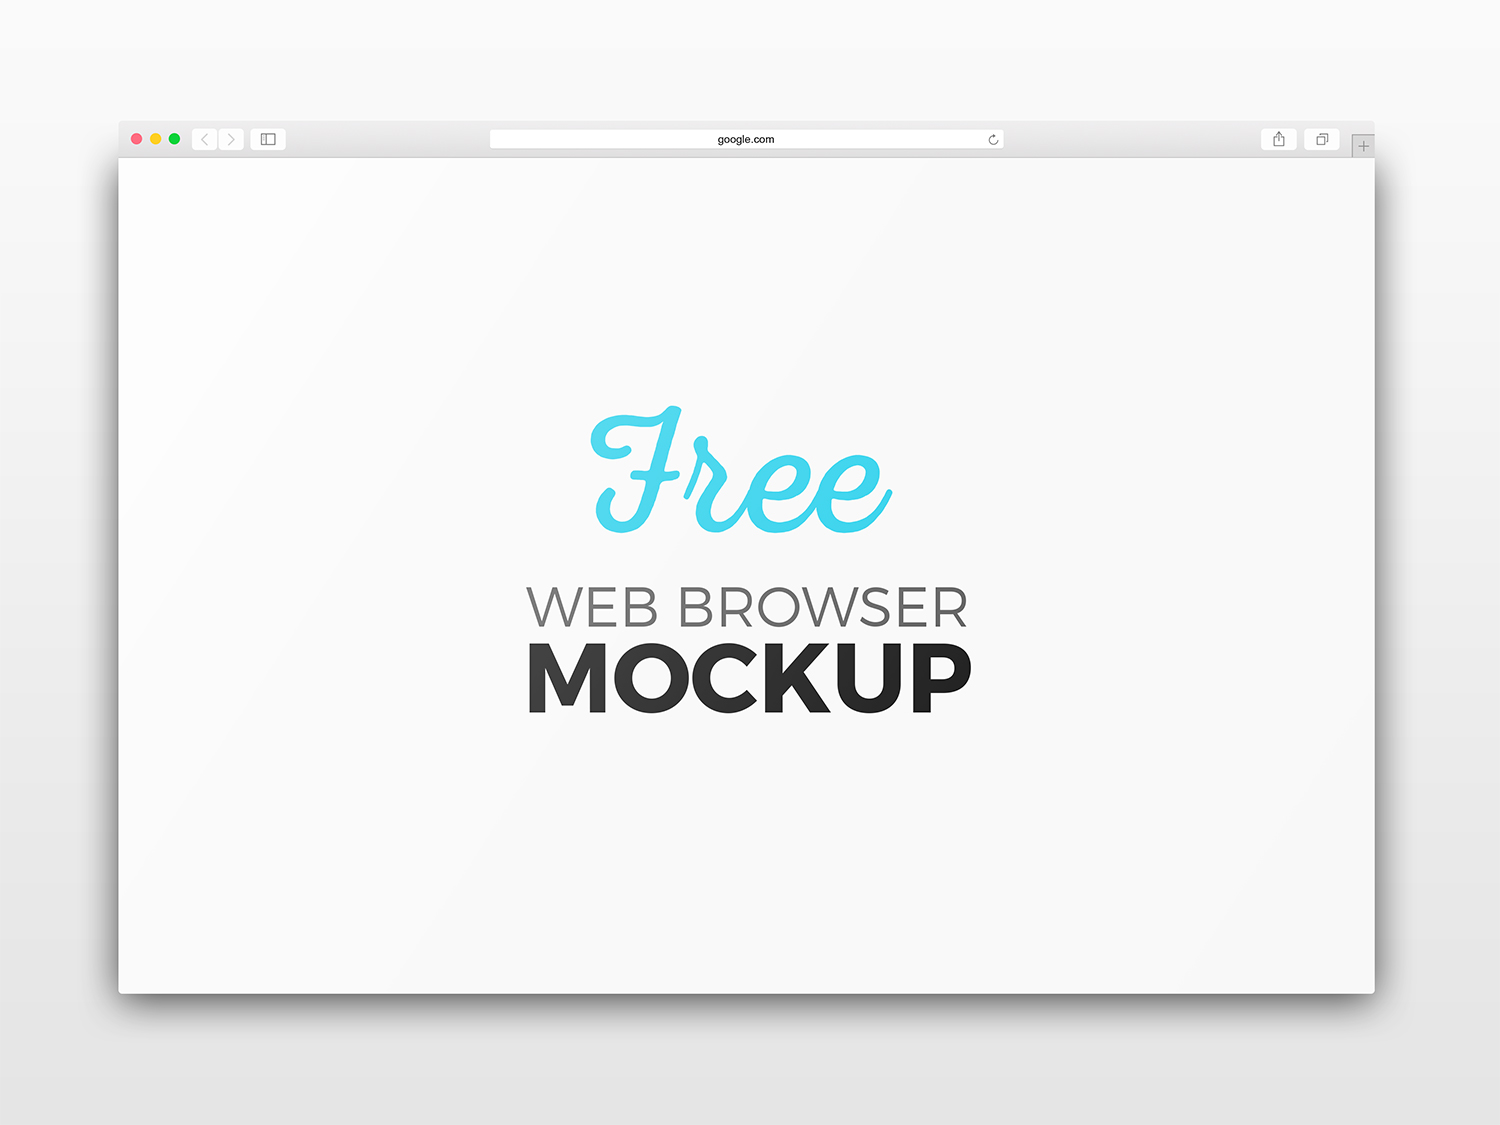
\includegraphics[width=\textwidth]{src/issues/1 - EXAMPLE/issue.jpg}
          \captionof{figure}{Vero repellat sed vero facere error ducimus et.}
          \label{1:EXAMPLE:issue.md:issue.jpg}
          \vspace{4ex}
        \end{minipage}
          
    \clearpage

    

\end{document}